\documentclass[a4paper,14pt]{extreport}
\usepackage[utf8]{inputenc}
\usepackage[english, russian]{babel}
\usepackage{listings}
\usepackage{graphicx}
\usepackage{float}
\graphicspath{{imgs/}}
\usepackage{amsmath,amsfonts,amssymb,amsthm,mathtools} 
\usepackage{pgfplots}
\usepackage{filecontents}
\usepackage{indentfirst}
\usepackage{eucal}
\usepackage{enumitem}
\frenchspacing

\usepackage{indentfirst} % Красная строка

\usetikzlibrary{datavisualization}
\usetikzlibrary{datavisualization.formats.functions}

\usepackage{amsmath}
\usepackage{fixltx2e}
\usepackage{caption}

\definecolor{bluekeywords}{rgb}{0,0,1}
\definecolor{greencomments}{rgb}{0,0.5,0}
\definecolor{redstrings}{rgb}{0.64,0.08,0.08}
\definecolor{xmlcomments}{rgb}{0.5,0.5,0.5}
\definecolor{types}{rgb}{0.17,0.57,0.68}

\usepackage{listings}
\lstset{language=[Sharp]C,
	captionpos=t,
	numbers=left, %Nummerierung
	numberstyle=\small, % kleine Zeilennummern
	frame=single, % Oberhalb und unterhalb des Listings ist eine Linie
	stepnumber=1,                   
	numbersep=5pt,                
	showspaces=false,
	tabsize=2,
	showtabs=false,
	breaklines=true,
	showstringspaces=false,
	breakatwhitespace=true,
	escapeinside={(*@}{@*)},
	commentstyle=\color{greencomments},
	morekeywords={partial, var, value, get, set},
	keywordstyle=\color{bluekeywords},
	stringstyle=\color{redstrings},
	basicstyle=\ttfamily\small,
}

\usepackage[left=3cm,right=1cm, top=2cm,bottom=2cm,bindingoffset=0cm]{geometry}
% Для измененных титулов глав:
\usepackage{titlesec, blindtext, color} % подключаем нужные пакеты
\definecolor{gray75}{gray}{0.75} % определяем цвет
\newcommand{\hsp}{\hspace{20pt}} % длина линии в 20pt
% titleformat определяет стиль
\titleformat{\chapter}[hang]{\Huge\bfseries}{\thechapter\hsp\textcolor{gray75}{|}\hsp}{0pt}{\Huge\bfseries}

\usepackage{array}
\newcommand{\head}[2]{\multicolumn{1}{>{\centering\arraybackslash}p{#1}}{#2}}



\begin{document}
	
\renewcommand{\contentsname}{Содержание}
\tableofcontents
\setcounter{page}{3}


\chapter*{Введение}
\addcontentsline{toc}{chapter}{Введение}

Методы прогнозирования многообразны, как и объекты, прогнозированием которых занимается человек. Ему всегда было интересно узнать будущее -- свое, своих близких, государства, экономики, предугадать погоду, определить как изменятся в ближайшее время курсы валют и т. п.

Но прогнозировать ситуацию важно не только из-за того, что это интересно, но и потому, что от предвидения будущего зависят действия человека. Если прогнозируется скачок цен на какой-то товар, то можно заранее закупить его. Можно сказать, что жизнь современного человека невозможно себе представить без прогнозирования.

Прогноз -- это результат индуктивного вывода, когда по характеру ограниченного множества значений показателей или взаимосвязи факторов делается вывод о том, что и остальные, еще не наблюдаемые значения этих показателей или взаимосвязи будут обладать аналогичными свойствами \cite{hse_pred}.

В мировой экономической науке накоплен и апробирован значительный арсенал методов прогнозирования, который дает возможность решать комплекс задач по обоснованию решений в различных областях \cite{bel_prog}.

Задача прогнозирования цен на потребительские товары актуальна для различных типов пользователей: во-первых, это конечные покупатели, которые принимают решение о покупке того или иного товара; прогноз цены может повлиять не только на выбор момента покупки, но и на сам факт покупки товара как таковой; во-вторых, это владельцы магазинов (необязательно онлайн), которые планируют закупки и ассортимент товаров; в-третьих, маркетологи, формирующие аналитику изменения рынка тех или иных товаров \cite{met_pred_online}.

Цель работы -- реализовать базу данных, хранящую информацию о покупателях, магазинах, ассортименте товаров в магазинах и историях цен товаров в них, и программное обеспечение для работы с информацией из этой базы данных, а также прогнозирования цен на товары в магазинах посредством построения линии тренда на основе истории цен.

Таким образом, необходимо решить следующие задачи:

\begin{itemize}
	\setlength\itemsep{0.01em}
	\item проанализировать варианты представления данных и выбрать из них подходящий для решения задачи;
	\item проанализировать системы управления базами данных и выбрать подходящую систему для хранения данных;
	\item проанализировать методы построения линии тренда и выбрать подходящий метод для прогнозирования цен;
	\item спроектировать базу данных, описать её сущности и связи;
	\item реализовать интерфейс для работы с базой данных;
	\item реализовать возможность построения линии тренда для прогнозирования цен на товары в магазинах;
	\item исследовать, к чему стремится значение цены товара на следующий месяц при увеличении выборки истории цен.
\end{itemize}
	
\chapter{Аналитический раздел}

В данном разделе формализованы данные, хранимые в базе данных, описана ролевая модель, описаны существующие системы управления базами данных и методы построения линии тренда.

\section{Формализация данных}

База данных должна хранить информацию о:

\begin{itemize}
	\setlength\itemsep{0.01em}
	\item магазинах;
	\item товарах
	\item ассортименте товаров в магазинах;
	\item историю цен на товары в магазинах за последние полтора года;
	\item товарные чеки.
\end{itemize}

ER-диаграмма сущностей базы данных представлена на рисунке \ref{db_proj}.

\begin{figure}[H]
	\centering
	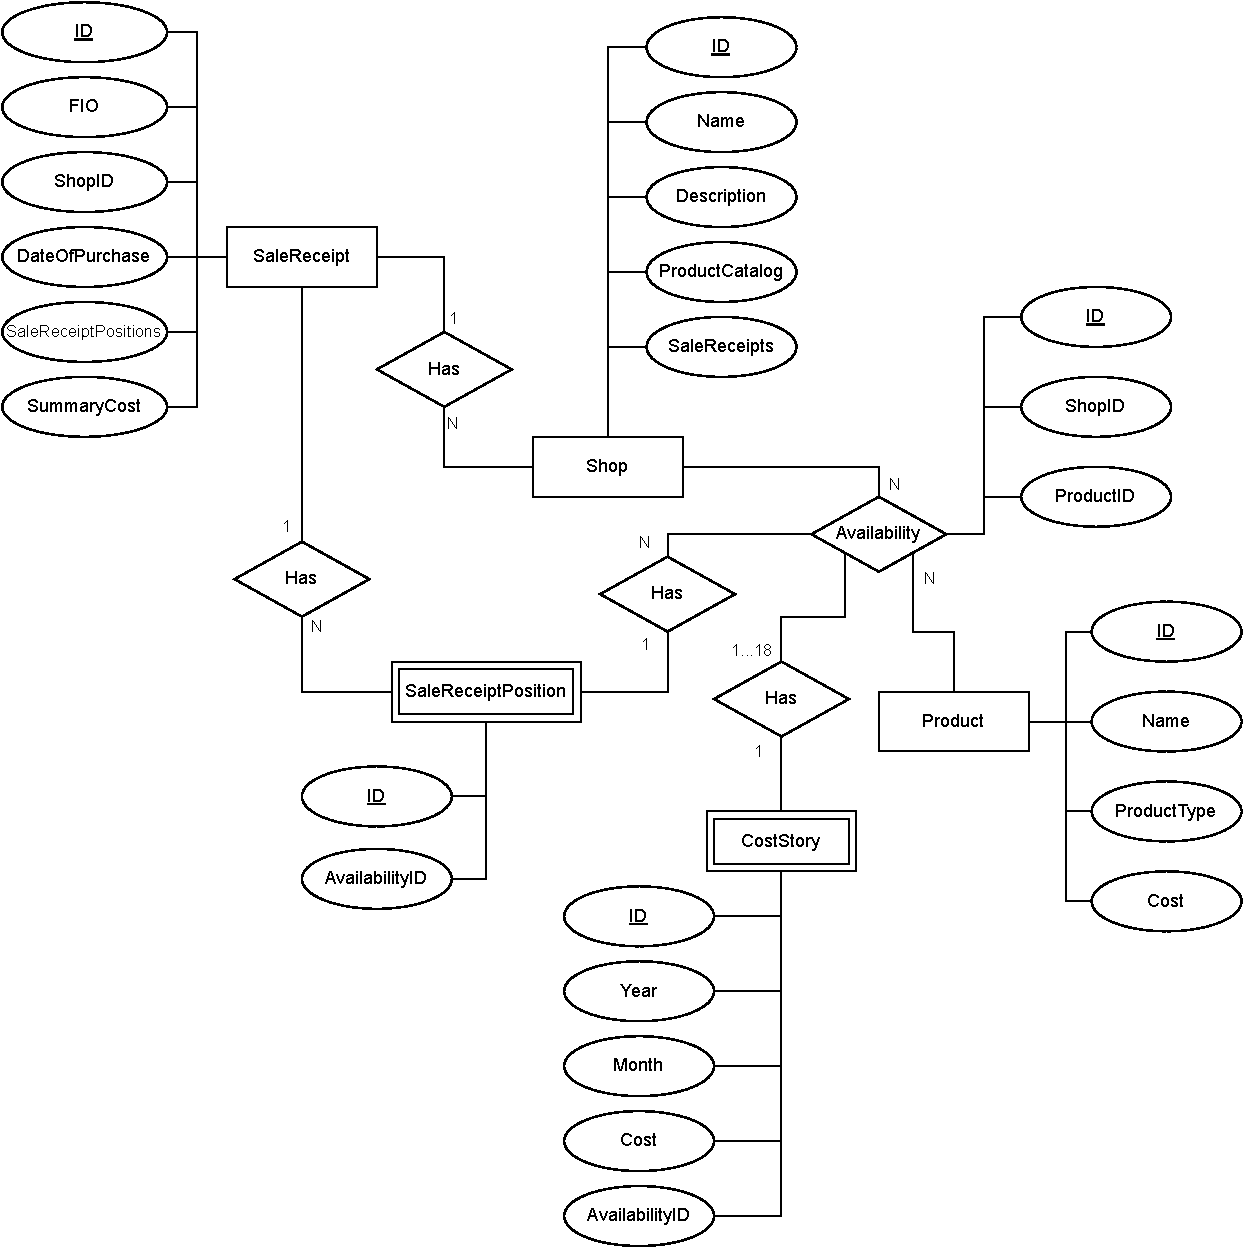
\includegraphics[scale=0.8]{ER.drawio.pdf}
	\caption{ER-диаграмма сущностей базы данных в нотации Чена.}
	\label{db_proj}
\end{figure}

\captionsetup[table]{skip=-12pt}
\captionsetup{singlelinecheck = false, justification=raggedright}
\begin{table}[H]
	\caption{Категории и описание данных}
	\begin{center}
		\begin{tabular}{| l | p{11 cm} |} 
			\hline
			
			\textbf{Категория} & \textbf{Описание} \\  
			
			\hline
			
			Магазин & Название, описание магазина, ассортимент товаров \\
			
			\hline
			
			Товар & Название, тип товара, актуальная цена \\
			
			\hline
			
			Ассортимент товаров & Список товаров \\
			
			\hline
			
			История цен & Год, месяц, цена в этот период \\
			
			\hline
			
			Товарный чек & ФИО, дата покупки, информация о месте покупки(магазине), список купленных товаров, итоговая стоимость \\
			\hline
		\end{tabular}
	\end{center}
\end{table}

На рисунке \ref{use_case} представлена Use-case-диаграмма ПО.

\captionsetup{singlelinecheck = false, justification=centering}
\begin{figure}[H]
	\centering
	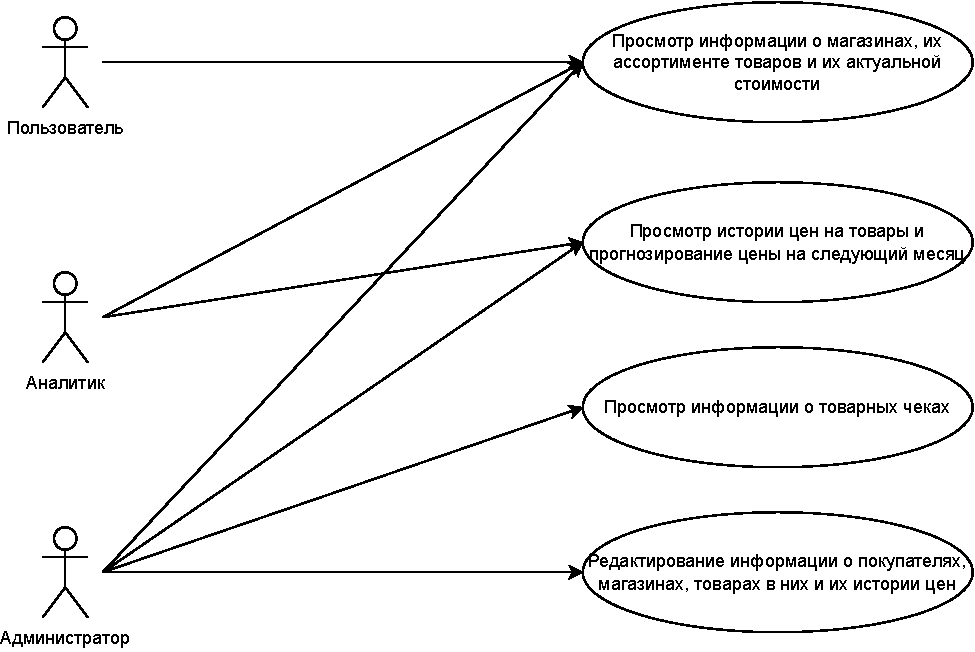
\includegraphics[scale=0.8]{use_case.drawio.pdf}
	\caption{Use-case-диаграмма ПО.}
	\label{use_case}
\end{figure}

\section{Описание ролевой модели}

Для управления системой введено три роли: пользователь, аналитик, администратор.

\begin{table}[H]
	\caption{Роли и описание их функционала}
	\begin{center}
		\begin{tabular}{| l | p{12 cm} |} 
			\hline
			
			\textbf{Роль} & \textbf{Функционал} \\  
			
			\hline
			
			Пользователь & Просмотр информации о магазинах, их ассортименте товаров и их актуальной стоимости \\
			
			\hline
			
			Аналитик & Просмотр информации о магазинах, их ассортименте товаров и их истории цен. Возможность прогнозирования цены на товар в магазине \\
			
			\hline
			
			Администратор & Просмотр, добавление и удаление информации о магазинах, их ассортименте товаров и их истории цен, товарных чеках. Возможность прогнозирования цены на товар в магазине \\
			
			\hline
		\end{tabular}
	\end{center}
\end{table}

Для доступа к ролям <<Аналитик>> и <<Администратор>> требуется авторизация (ввод пароля).

\section{Обзор существующих СУБД}

Система управления базами данных (сокр. СУБД) -- Программная система, предназначенная для создания и хранения базы данных на основе некоторой модели данных, обеспечения логической и физической целостности содержащихся в ней данных, надежного и эффективного использования ресурсов (данных, пространства памяти и вычислительных ресурсов), предоставления к ней санкционированного доступа для приложений и конечных пользователей, а также для поддержки 
функций администратора базы данных \cite{kogal}.

""\newline
Функции СУБД:

\begin{itemize}
	\setlength\itemsep{0.01em}
	\item управление данными во внешней памяти;
	\item управление данными в оперативной памяти с использованием дискового кэша;
	\item журнализация изменений, резервное копирование и восстановление базы данных после сбоев;
	\item поддержка языков БД.
\end{itemize}

\subsection{Классификация СУБД по модели данных}

Модель данных --  система типов данных, типов связей между ними и допустимых видов ограничений целостности, которые могут быть для них определены. Здесь имеется в виду современное понимание типа данных как носителя свойств, определяющих и состояние экземпляров типа, и их поведение \cite{kogal}.

По этому признаку СУБД делят на:

\begin{itemize}
	\setlength\itemsep{0.01em}
	\item дореляционные;
	\item реляционные;
	\item постреляционные.
\end{itemize}


\subsection*{Дореляционные СУБД}

К ним относятся иерархические и сетевые СУБД.

""\newline
\noindent\textbf{Иерархические СУБД}

В иерархических СУБД используется представление базы данных в виде древовидной (иерархической) структуры, состоящей из объектов (данных) различных уровней.

Между объектами существуют связи, каждый объект может включать в себя несколько объектов более низкого уровня. Такие объекты находятся в отношении предка (объект более близкий к корню) к потомку (объект более низкого уровня), при этом возможна ситуация, когда объект-предок не имеет потомков или имеет их несколько, тогда как у объекта-потомка обязательно только один предок. Объекты, имеющие общего предка, называются близнецами \cite{scienceforum}.

Примеры: Caché, Google App Engine Datastore API.

""\newline
\noindent\textbf{Сетевые СУБД}

Сетевые СУБД подобны иерархическим, за исключением того, что в них имеются указатели в обоих направлениях, которые соединяют родственную информацию.

Несмотря на то, что эта модель решает некоторые проблемы, связанные с иерархической моделью, выполнение простых запросов остается достаточно сложным процессом.

Также, поскольку логика процедуры выборки данных зависит от физической организации этих данных, то эта модель не является полностью независимой от приложения. Другими словами, если необходимо изменить структуру данных, то нужно изменить и приложение \cite{scienceforum}.

Примеры: Caché.

\subsection*{Реляционные СУБД}

Реляционные СУБД ориентированы на организацию данных в виде двумерных таблиц. Каждая реляционная таблица представляет собой двумерный массив и обладает следующими свойствами:

\begin{enumerate}
	\setlength\itemsep{0.01em}
	\item каждый элемент таблицы является одним элементом данных;
	\item каждый столбец обладает своим уникальным именем;
	\item одинаковые строки в таблице отсутствуют;
	\item все столбцы в таблице однородные, то есть все элементы в столбце имеют одинаковый тип;
	\item порядок следования строк и столбцов может быть произвольным.
\end{enumerate}

Практически все разработчики современных приложений, предусматривающих связь с системами баз данных, ориентируются на реляционные СУБД. По оценке Gartner в 2013 году рынок реляционных СУБД составлял 26 млрд долларов с годовым приростом около 9\%, а к 2018 году рынок реляционных СУБД достигнет 40 млрд долларов. В настоящее время абсолютными лидерами рынка СУБД являются компании Oracle, IBM и Microsoft, с общей совокупной долей рынка около 90\%, поставляя такие системы как Oracle Database, IBM DB2 и Microsoft SQL Server \cite{dbms}.


\subsection*{Постреляционные СУБД}

Постреляционная модель является расширением реляционной модели. Она снимает ограничение неделимости данных, допуская многозначные поля, значения которых состоят из подзначений, и набор значений воспринимается как самостоятельная таблица, встроенная в главную таблицу \cite{post_rel}.

С ним относятся объектно-ориентированные и объектно-реляционные СУБД.

""\newline
\noindent\textbf{Объектно-ориентированные СУБД}

Объектно-ориентированные СУБД управляют базами данных, в которых данные моделируются в виде объектов, их атрибутов, методов и классов.

Этот вид СУБД позволяет работать с объектами баз данных так же, как с объектами в программировании в объектно-ориентированных языках программирования. ООСУБД расширяет языки программирования, прозрачно вводя долговременные данные, управление параллелизмом, восстановление данных, ассоциированные запросы и другие возможности  \cite{dbms}.

Примеры: GemStone.

""\newline
\noindent\textbf{Объектно-реляционные СУБД}

Объектно-реляционные СУБД поддерживают некоторые технологии, реализующие объектно-ориентированный подход: объекты, классы и наследование реализованы в структуре баз данных и языке запросов.

Зачастую все те СУБД, которые называются реляционными, являются, по факту, объектно-реляционными \cite{dbms}.

В данной работе будет рассмотрен имено этот класс СУБД.

Примеры: PostgreSQL, DB2, Oracle Database, Microsoft SQL Server.


\subsection{Обзор объектно-реляционных СУБД}

\subsubsection*{Oracle Database}

Oracle Database \cite{orc_db} -- объектно-реляционная система управления базами данных компании Oracle \cite{orc}.

На данный момент у этого продукта блестящая репутация \cite{cmp_db}. Кроме того, существует несколько версий этого продукта для удовлетворения потребностей конкретной организации.

Актуальная версия Oracle на данный момент предназначена для облачных сред и может быть размещена на одном или нескольких серверах, это позволяет управлять базами данных, которые содержат миллиарды записей. Некоторые из функций новейшей версии Oracle включают в себя grid framework и использования как физических, так и логических структур.

Это означает, что физическое управление данными не влияет на доступ к логическим структурам. Кроме того, безопасность в этой версии доведена до высочайшего уровня, потому что каждая транзакция изолирована от других.

\subsubsection*{Microsoft SQL Server}

Microsoft SQL Server \cite{mssql} -- система управления реляционными базами данных (РСУБД), разработанная корпорацией Microsoft.

Microsoft SQL Server является ещё одной из популярных СУБД \cite{cmp_db}. Это система управления базами данных, движок которой работает на облачных серверах, а также локальных серверах, причем можно комбинировать типы применяемых серверов одновременно. Вскоре после выпуска Microsoft SQL Server 2016, Microsoft адаптировала продукт для операционной системы Linux, а на платформе Windows он работал изначально.

Одной из уникальных особенностей версии 2016 года является temporal data support (временная поддержка данных), которая позволяет отслеживать изменения данных с течением времени. Последняя версия Microsoft SQL-сервер поддерживает dynamic data masking (динамическую маскировку данных), которая гарантирует, что только авторизованные пользователи будут видеть конфиденциальные данные.

\subsubsection*{PostgreSQL}

PostgreSQL \cite{pg} -- свободная объектно-реляционная система управления базами данных (СУБД).

PostgreSQL является одним из нескольких бесплатных популярных вариантов СУБД, часто используется для ведения баз данных веб-сайтов \cite{cmp_db}. Это весьма старая система, поэтому в настоящее время она хорошо развита, и позволяет пользователям управлять как структурированными, так и неструктурированными данными. Может быть использована на большинстве основных платформ, включая Linux (где особенно хорошо проявляется производительность). Прекрасно справляется с задачами импорта информации из других типов баз данных с помощью собственного инструментария.

Движок БД может быть размещен в ряде сред, в том числе виртуальных, физических и облачных. Последняя версия PostgreSQL предлагает обработку больших объемов данных и увеличение числа одновременно работающих пользователей. Безопасность была улучшена благодаря поддержке DBMS\_SESSION.

\subsubsection*{DB2}

DB2 \cite{db2} -- семейство систем управления реляционными базами данных, выпускаемых корпорацией IBM. Чаще всего, ссылаясь на DB2, имеют в виду реляционную систему управления базами данных DB2 Universal Database (DB2 UDB).

DB2 представляет собой СУБД, которая имеет возможности NoSQL, и может читать JSON и XML-файлы  \cite{cmp_db}. Ввиду того, что система разрабатывалась для серверов компании IBM модельного ряда iSeries, логично, что система работает на Windows, Linux и MacOS.

Диалект языка SQL, используемый в DB2 за редкими исключениями строго декларативен, система снабжена многофазовым оптимизатором, строящим по этим декларативным конструкциям план выполнения запроса.

Оптимизатор DB2 широко использует статистику распределения данных в таблицах (если процесс её сбора был выполнен администратором базы данных), поэтому один и тот же запрос на языке SQL может быть оттранслирован в совершенно различные планы выполнения в зависимости от статистических характеристик данных, которые он обрабатывает.

Одно из улучшений DB2 -- Blu Acceleration, которое предназначено для ускорения работы базы данных. Пропуск данных предназначен для повышения быстродействия системы с большим количеством данных, чем может она может вместить в себя. Последняя версия DB2 также обеспечивает усовершенствованные функции аварийного восстановления, совместимости и аналитики.


\section{Методы построения линии тренда}

Линия тренда -- прямая или кривая линия, аппроксимирующая (приближающая) исходные данные на основе уравнения регрессии или скользящего среднего \cite{lt_exel}. Аппроксимация определяется по ме­тоду наименьших квадратов \cite{mnk}. В зависимости от характера поведения исходных данных (убыва­ют, возрастают и т.д.) выбирается метод интерполяции, который сле­дует использовать для построения тренда.

\subsection{Виды линий трендов}

\subsubsection*{Линейная линия тренда}

Линейная линия тренда определяется функцией

\begin{equation}
	y = ax + b,
\end{equation}

где $a$ -- тангенс угла наклона прямой, $b$ -- смещение.

Прямая линия тренда (линейный тренд) наилучшим образом подходит для величин, изменяющихся с постоянной скоростью. Приме­няется в случаях, когда точки данных расположены близко к прямой \cite{lt_exel}.

\subsubsection*{Логарифмическая линия тренда}

Логарифмическа линия тренда определяется функцией

\begin{equation}
	y = a\ln x + b,
\end{equation}

где $a$ и $b$ -- константы.

Логарифмическая линия тренда соответствует ряду данных, значения которого вначале быстро растут или убывают, а затем постепенно стабилизируются. Может использоваться для положительных и отрицательных данных \cite{lt_exel}.

\subsubsection*{Полиномиальная линия тренда}

Полиномиальная линия тренда определяется функцией

\begin{equation}
	y = \sum_{i = 0}^{n} a_i x^i, n \leqslant 6,
\end{equation}

где $a_i$ -- коэффициенты полинома.

Полиномиальная линия тренда используется для описания попеременно возрастающих и убывающих данных. Степень полинома подбирают таким образом, чтобы она была на единицу больше количества экстремумов (максимумов и минимумов) кривой \cite{lt_exel}.

\subsubsection*{Экспоненциальная линия тренда}

Экспоненциальная линия тренда определяется функцией

\begin{equation}
	y = a e ^ {bx},
\end{equation}

где $a$ и $b$ -- константы.

Экспоненциальный тренд используется в случае непрерывного возрастания изменения данных. Построение указанного тренда не­возможно, если в множестве значений членов ряда присутствуют нулевые или отрицательные данные \cite{lt_exel}.

\subsubsection*{Степенная линия тренда}

Степенная линия тренда определяется функцией

\begin{equation}
	y = a x ^ b,
\end{equation}

где $a$ и $b$ -- константы.

Степенная линия тренда дает хорошие результаты для положительных данных с постоянным ускорением. Для рядов с нулевыми или отрицательными значениями построение указанной линии трен­да невозможно \cite{lt_exel}.

\subsubsection*{Линейная фильтрация}

Линейная фильтрация определяется формулой

\begin{equation}
	F_t = \frac{A_t + A_{t-1} + ... + A_{t-n+1}}{n}, (2 \leqslant t < n),
\end{equation}

где $n$ -- общее число членов ряда, $t$ -- параметр фильтра.

Тренд с линейной фильтрацией позволяет сгладить колебания данных, наглядно демонстрируя характер зависимостей \cite{lt_exel}. Для построения указанной линии тренда пользователь должен задать число $t$.

Линейная фильтрация использует метод скользящего среднего, при котором каждое значение функции заменяется средним арифметическим $A$ по $t$ соседним точкам, расположенным симметрично относительно данной. Линия тренда в этом случае уравнения не имеет \cite{lin_filt}, поэтому для прогноза изменения величины она не подходит.

\subsection{Анализ исходных данных для построения линии тренда}

Цена товара как величина положительная и имеет непостоянный рост: она может как расти, так и падать. Таким образом, для прогнозирования цен на товары подходит полиномиальная линия тренда.

\section*{Вывод к аналитическому разделу}
\addcontentsline{toc}{section}{Вывод к аналитическому разделу}

В данном разделе были формализованы данные, хранимые в базе данных, описана ролевая модель, рассмотрены существующие СУБД и методы построения линии тренда.



\chapter{Конструкторский раздел}

\section{Проектирование базы данных}

В базе данных существует 6 таблиц, одна из которых является развязочной (Availability). Остальные таблицы на диаграмме представлены в виде сущностей. На рисунке \ref{db} представлена ER-диаграмма сущностей БД.

\begin{figure}[H]
	\centering
	\includegraphics[scale=0.8]{}
	\caption{ER-диаграмма сущностей БД.}
	\label{db}
\end{figure}

Таблица \textbf{Shop} хранит данные о магазинах и содержит следующие поля:
\begin{itemize}
	\setlength\itemsep{0.01em}
	\item ID -- идентификатор магазина;
	\item Name -- название магазина;
	\item Description -- описание магазина.
\end{itemize}

""\newline\indent
Таблица \textbf{Product} хранит данные о продуктах и содержит следующие поля:
\begin{itemize}
	\setlength\itemsep{0.01em}
	\item ID -- идентификатор продукта;
	\item Name -- название продукта;
	\item ProductType -- тип продукта.
\end{itemize}

""\newline\indent
Таблица \textbf{Availability} хранит отношения наличия товара в каталоге магазина и содержит следующие поля:
\begin{itemize}
	\setlength\itemsep{0.01em}
	\item ID -- идентификатор отношения;
	\item ShopID -- идентификатор магазина;
	\item ProductID -- идентификатор продукта.
\end{itemize}

""\newline\indent
Таблица \textbf{CostStory} хранит историю цен на товары в магазинах и содержит следующие поля:
\begin{itemize}
	\setlength\itemsep{0.01em}
	\item ID -- идентификатор значения цены в конкретный год и месяц;
	\item Year -- год;
	\item Month -- месяц;
	\item Cost -- значение цены в конкретный год и месяц;
	\item AvailabilityID -- идентификатор отношения наличия товара в каталоге магазина.
\end{itemize}

""\newline\indent
Таблица \textbf{SaleReceipt} хранит данные о товарных чеках и содержит следующие поля:
\begin{itemize}
	\setlength\itemsep{0.01em}
	\item ID -- идентификатор товарного чека;
	\item FIO -- ФИО покупателя;
	\item ShopID -- идентификатор магазина, в котором была совершена покупка;
	\item DateOfPurchase -- дата покупки.
\end{itemize}

""\newline\indent
Таблица \textbf{SaleReceiptPosition} хранит информацию о позиции в чеке и содержит следующие поля:
\begin{itemize}
	\setlength\itemsep{0.01em}
	\item ID -- идентификатор позиции чека;
	\item AvailabilityID -- идентификатор отношения наличия товара в каталоге магазина.
\end{itemize}

""\newline\indent
Таблицы \textbf{SaleReceiptPosition} и \textbf{CostStory} содержат поле идентификатора отношения наличия товара в каталоге магазина в целях борьбы с рассинхронизацией: товарный чек и история цен на товар в магазине не могут ссылаться на товары, которых нет в данном магазине.

Актуальная стоимость товара в магазине формируется как последнее по дате значение цены товара в истории цен.


\section*{Вывод к конструкторскому разделу}
\addcontentsline{toc}{section}{Вывод к конструкторскому разделу}

\chapter{Технологический раздел}

\section{Средства реализации}

Для решения задачи была выбрана СУБД PostgreSQL, т. к. она открытая, кросплатформенная, имеет поддержку БД неограниченного размера, мощные и надёжные механизмы транзакций и репликации, систему встроенных языков программирования (PL/pgSQL \cite{plpgsql}, plpython3u \cite{plpython3u}), а также легкую расширяемость.

\section*{Вывод к технологическому разделу}
\addcontentsline{toc}{section}{Вывод к технологическому разделу}

\chapter{Экспериментально-исследовательский раздел}

\section*{Вывод к экспериментально-исследовательскому разделу}
\addcontentsline{toc}{section}{Вывод к экспериментально-исследовательскому разделу}

\chapter*{Заключение}
\addcontentsline{toc}{chapter}{Заключение}


\newpage
\addcontentsline{toc}{chapter}{Список литературы}
\renewcommand\bibname{Список литературы}

\begin{thebibliography}{3}
	\bibitem{hse_pred} Методы и модели социально-экономического прогнозирования : учебник и практикум для академического бакалавриата. В 2-х т. Т. 1. Теория и методология прогнозирования / И. С. Светуньков, С. Г. Светуньков. — М. : Издательство Юрайт, 2014. — 351 с. — Серия : Бакалавр. Академический курс.
	
	\bibitem{bel_prog} Касперович С.А. Прогнозирование и планирование экономики : курс лекций для студентов специальностей 1-25 01 07 «Экономика и управление предприятием», 1-25 01 08 «Бухгалтерский учет, анализ и аудит», 1-26 02 02 «Менеджмент», 1-26 02 03 «Маркетинг» / С. А. Касперович. - Минск. : БГТУ, 2007. - 172 с. 
	
	\bibitem{met_pred_online} К. В. Богданов. Методика прогнозирования цен на товары в интернет-магазинах [Электронный ресурс]. -- Режим доступа: https://cyberleninka.ru/article/n/metodika-prognozirovaniya-tsen-na-tovary-v-internet-magazinah/viewer (дата обращения 4.04.2022)
	
	\bibitem{kogal} Когаловский М.Р. Энциклопедия технологий баз данных. — М.: Финансы и статистика, 2002. — 800 с.
	
	\bibitem{scienceforum} Классификация систем управления базами данных [Электронный ресурс]. -- Режим доступа: https://scienceforum.ru/2016/article/2016019197 (дата обращения 6.04.2022)
	
	\bibitem{dbms} Системы управления базами данных [Электронный ресурс]. -- Режим доступа: https://lecturesdb.readthedocs.io/databases/dbms.html (дата обращения 8.04.2022)
	
	\bibitem{post_rel} Постреляционная, многомерная и объектно-ориентированная модели данных [Электронный ресурс]. -- Режим доступа:  http://bseu.by/it/tohod/lekcii2\_4.htm?ysclid=l3njaseoko (дата обращения 8.04.2022)
	
	\bibitem{orc_db} Oracle Database [Электронный ресурс]. -- Режим доступа: https://www.oracle.com/database/ (дата обращения 8.04.2022)
	
	\bibitem{orc} Oracle [Электронный ресурс]. -- Режим доступа: https://www.oracle.com/ (дата обращения 8.04.2022)
	
	\bibitem{cmp_db} Сравнение современных СУБД [Электронный ресурс]. -- Режим доступа:  https://drach.pro/blog/hi-tech/item/145-db-comparison (дата обращения 8.04.2022)
	
	\bibitem{mssql} Microsoft SQL-Server  [Электронный ресурс]. -- Режим доступа:  https://www.microsoft.com/ru-ru/sql-server/sql-server-2019 (дата обращения 8.04.2022)
	
	\bibitem{pg} PostgreSQL [Электронный ресурс]. -- Режим доступа: https://www.postgresql.org/ (дата обращения 8.04.2022)
	
	\bibitem{plpgsql} PL/pgSQL [Электронный ресурс]. -- Режим доступа: https://www.postgresql.org/docs/9.6/plpgsql.html (дата обращения 8.04.2022)
	
	\bibitem{plpython3u} PL/Python [Электронный ресурс]. -- Режим доступа: https://www.postgresql.org/docs/current/plpython-python23.html (дата обращения 8.04.2022)
	
	\bibitem{db2} DB2 [Электронный ресурс]. -- Режим доступа: https://www.ibm.com/analytics/db2 (дата обращения 8.04.2022)
	
	\bibitem{lt_exel} Построение линии тренда в Excel [Электронный ресурс]. -- Режим доступа: https://ya-znau.ru/znaniya/zn/202 (дата обращения 9.04.2022)
	
	\bibitem{mnk} Линник Ю. В. Метод наименьших квадратов и основы математико-статистической теории обработки наблюдений. — 2-е изд. — М., 1962. (математическая теория)
	
	\bibitem{lin_filt} Линейная фильтрация [Электронный ресурс]. -- Режим доступа: https://poznayka.org/s23136t1.html (дата обращения 9.04.2022)
\end{thebibliography}
	
\end{document}